\chapter{Planning in Four Subspaces}%
\label{chap:proposed_planning}
\textit{This chapter presents an existing motion planner~\cite{chen_fast_2018} that is extended to incorporate movable and unknown spaces next to the conventional free and obstacle spaces. The modification incentivizes the planner to find a path in free space but can pass through unknown or movable space as a last resort. The robot should first remove the blocking objects if a planned path crosses an unknown or movable subspace.\bs}

Finding a path between the start- and target configuration whilst avoiding collisions was presented in previous chapter. Now that path planner is modified; the modification extends the planner to incorporate movable and unknown space. The modified algorithm has four tuning parameters that can be tweaked; The \textit{step size} and \textit{search size} were discussed in previous chapter. The third and fourth tuning parameters are the fixed costs for crossing through movable or unknown space. These cost are added to the \textit{TotalPathCost}, which is redefined as:\bs

\[\mathit{Cost_{path}} = \mathit{MovableSpaceCost} + \mathit{UnknownSpaceCost} \sum_{i=1}^{n-1} \mathit{Distance}(\gls{c}_i, \gls{c}_{i+1})\]
\todo{In the pseudoce you talk about objectCost, here totalpathCost, unclear!}

The \textit{MovableSpaceCost} and \textit{UnknownSpaceCost} correspond to a fixed addition cost for a configuration in the path that crosses through movable or unknown subspace, respectively. Crossing through is defined as one or more nodes in the path lying in that subspace. If a path does not contain a node in movable space, \textit{MovableSpaceCost} will be 0, equivalent to unknown space and \textit{UnknownSpaceCost}. Optimizing the path for the lowest cost incentives the path planning algorithm to find a path around unknown or movable objects.\bs

The added fixed cost for a path crossing through a movable or unknown object motivates the path planner to find the shortest path around objects but prefers moving an object over making a large detour. Tuning the additional fixed cost for a path crossing through movable or unknown space balances the robot's decision between the length of a detour the robot is willing to drive, compared to pushing an object to free the path. Removing an unknown object bears more uncertainty than a movable object, motivating a higher cost to remove an unknown object compared to an known object. In the following pseudocode for the modified path planner is presented, changes compared to previously shown pseudocode are indicated in red.\bs

The proposed algorithm prevents planning a path through blocking objects except when no other option is available or a large detour can be prevented. No performance tests have been conducted on the modified path planner, apart from visual inspection. \Cref{fig:mp_push_or_drive} clearly shows the effect of varying \textit{UnknownSpaceCosts}.

\newpage
\todo{eleborate on the change compared to the previous existing algorithm}
\todo{Dubble check if only the parts in red are changed.}
\begin{algorithm}[H]
  \caption{Pseudocode for modified \ac{RRT*} path planning algorithm. Lines that contain changes compared to \Cref{pseudocode:proposed_rrt_star_all} are indicated with the red colour.}%
  \label{pseudocode:modified_proposed_rrt_star}
  \begin{algorithmic}[1]
    \State $\gls{nodesMP} \leftarrow x_{init}$
    \While{\textit{NotReachStop}}
        \State $\gls{nodeMP}_\mathit{rand} \leftarrow \mathit{Sample_{random}}$ \algorithmiccomment{Create, project and validate a new random sample}
      \State $\gls{nodeMP}_\mathit{nearest} \leftarrow \mathit{Nearest(\gls{nodeMP}_{rand}, \gls{nodesMP})}$
      \State $\gls{nodeMP}_\mathit{temp} \leftarrow \mathit{Project(\gls{nodeMP}_{rand}, \gls{nodeMP}_{nearest})}$
      \If{$\mathit{CollisionCheck(\gls{nodeMP}_{temp})}$}
      \State $\gls{nodeMP}_\mathit{new} = \gls{nodeMP}_\mathit{temp}$
      \State $\mathit{Cost_{toInitMin}} \leftarrow +\infty$ 
      \Else
      \State Continue
      \EndIf
      \State $X_\mathit{near} \leftarrow \mathit{NearestSet(\gls{nodeMP}_{new}, \gls{nodesMP})}$ \algorithmiccomment{Find and connect new node to parent node}
      \For{$\gls{nodeMP}_\mathit{near} \in X_\mathit{near}$}
    \State $\mathit{Cost_{temp}} \leftarrow \mathit{CostToInit}(\gls{nodeMP}_\mathit{near}) + \mathit{Distance}(\gls{nodeMP}_\mathit{near}, \gls{nodeMP}_\mathit{new}) + \textcolor{red}{\mathit{ObjectCost}(\gls{nodeMP}_\mathit{near}, \gls{nodeMP}_\mathit{new})}$
      \If{$\mathit{Cost_{temp}}  < \mathit{Cost_{toInitMin}}$}
      \State $\mathit{Cost_{toInitMin}} \leftarrow \mathit{Cost_{new}}$
      \State $\gls{nodeMP}_\mathit{minCost} \leftarrow \gls{nodeMP}_\mathit{near}$
      \EndIf
      \EndFor
      \If{$\mathit{Cost_{toInitMin}} == \infty$}
          \State Continue
      \Else
      \State $\gls{nodesMP}.add(\gls{nodeMP}_\mathit{new})$
      \State $E.\mathit{add}(\gls{nodeMP}_\mathit{minCost}, \gls{nodeMP}_\mathit{new})$
      \EndIf
      \State $\mathit{Cost_{pathMin}} \leftarrow +\infty$ 
      \For{$\gls{nodeMP}_\mathit{near} \in X_{near}$}\algorithmiccomment{\parbox[t]{.6\linewidth}{Check if the newly added node can lower cost for nearby nodes and if a both connectivity trees can be connected}}
      \If{$\mathit{InSameTree(\gls{nodeMP}_{near}, \gls{nodeMP}_{new})}$}
    \If{$\mathit{CostToInit(\gls{nodeMP}_{new})} + \mathit{Distance(\gls{nodeMP}_{new}, \gls{nodeMP}_{near})} +\textcolor{red}{\mathit{ObjectCost}(\gls{nodeMP}_\mathit{new}, \gls{nodeMP}_\mathit{near})} < \mathit{CostToInit(\gls{nodeMP}_{near})}$}
      \State $\mathit{E.rewire(\gls{nodeMP}_{near}, \gls{nodeMP}_{new})}$
      \EndIf
      \Else \algorithmiccomment{Add lowest cost path to the list of paths}

      \State $\mathit{Cost_{temp} \leftarrow CostToInit(\gls{nodeMP}_{new}) + Distance(\gls{nodeMP}_{new}, \gls{nodeMP}_{near})} + \mathit{CostToInit(\gls{nodeMP}_{near})}$
      % \State $\mathit{Cost_{temp} \leftarrow CostToInit(\gls{nodeMP}_{new}) + Distance(\gls{nodeMP}_{new}, \gls{nodeMP}_{near})} + \mathit{CostToInit(\gls{nodeMP}_{near}) + \textcolor{red}{ObjectCost(\gls{nodeMP}_{new}, \gls{nodeMP}_{near})}}$
      \If{$\mathit{Cost_{temp}  < Cost_{pathMin}}$}
      \State $\mathit{Cost_{pathMin}} \leftarrow \mathit{Cost_{temp}}$
      \State $\mathit{\gls{nodeMP}_{pathMin} \leftarrow \gls{nodeMP}_{near}}$
      \EndIf
      \EndIf
      \If{$Cost_{pathMin} == \infty$}
      \State Continue
      \Else
      \State $\mathit{P.addPath(\gls{nodeMP}_{new}, \gls{nodeMP}_{pathMin}, Cost_{pathMin})}$
      \EndIf
      \EndFor
    \EndWhile
  \end{algorithmic}
\end{algorithm}

\begin{figure}[H]
    \centering
    \begin{subfigure}{\textwidth}
    \centering
    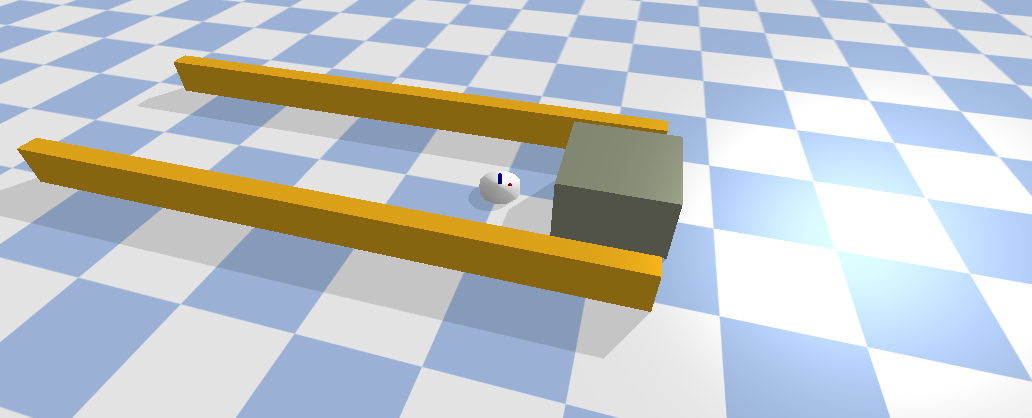
\includegraphics[width=0.8\textwidth]{figures/required_background/push_or_drive} \caption{Robot environment with the point robot, two yellow unmovable walls and an unknown brown box.\\The robot tasked to drive toward the opposite side of the brown box.}

\todo{Could you at least place a ghost pose on in this figure?}

    \end{subfigure}

    \begin{subfigure}{1.11\textwidth}
    \centering
    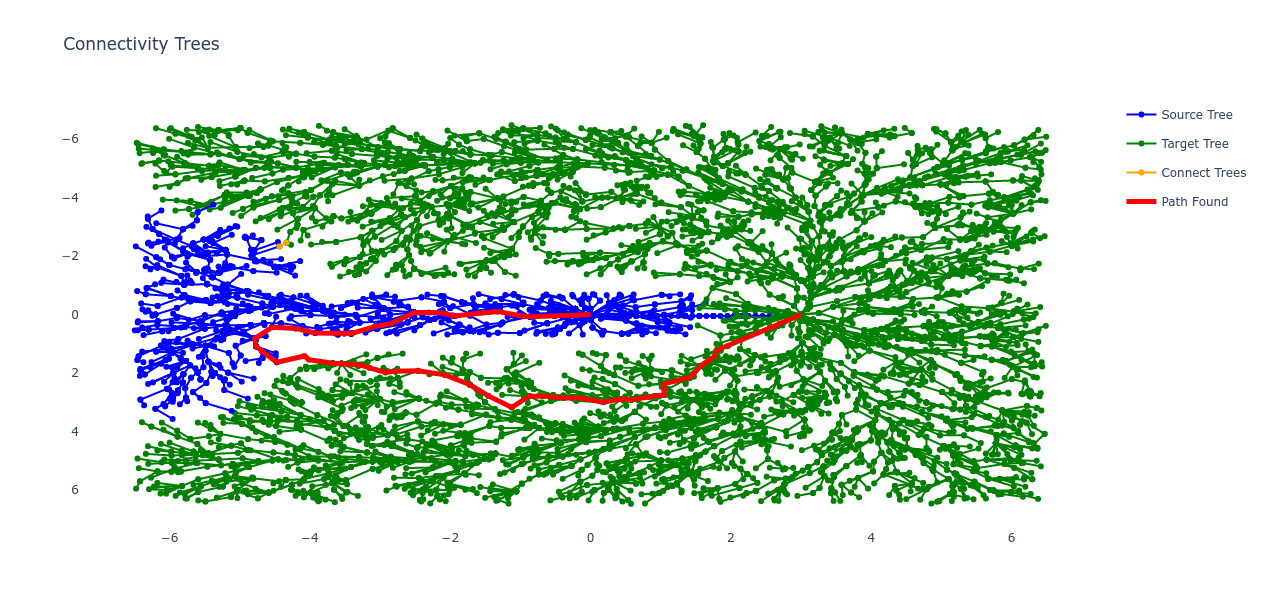
\includegraphics[width=\textwidth]{figures/required_background/mp/mp_high_fixed_cost}
    \caption{Visualization of the planned path around the brown box and yellow obstacles, with $\mathit{UnknownSpaceCost} = 1$.}
    \end{subfigure}

    \begin{subfigure}{1.11\textwidth}
    \centering
    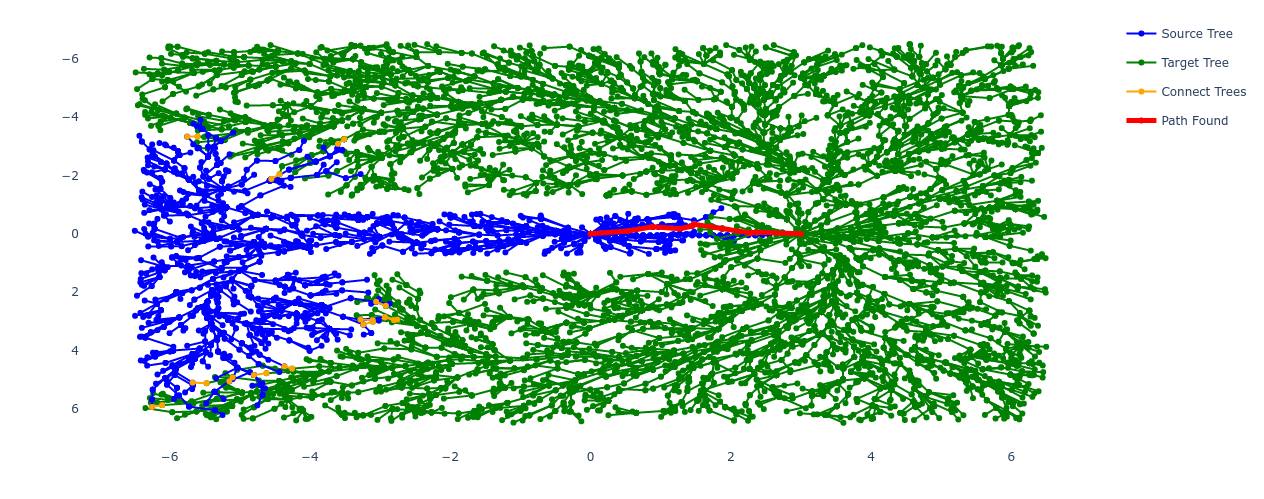
\includegraphics[width=\textwidth]{figures/required_background/mp/mp_low_fixed_cost}
    \caption{Visualization of the planned path going through the brown box, $\mathit{UnknownSpaceCost} = 0.5$.}
    \end{subfigure}
    \caption{Driving task and two path planned by the modified planning algorithm.}%
    \label{fig:mp_push_or_drive}
\end{figure}

Now that the modified path planner is discussed, the proposed robotic framework is discussed. The proposed framework relies on the required background from previous chapter, and relies on the modified path planner from this chapter.\bs



\todo{create a test that does things for the boxer robot, and it must have nonholonomic checker residing in the path}


% old manipulation section shit

% \subsection{Manipulation Planning}%
% \label{subsec:manipulation_planning}
% With a push, two objects are primarily involved, the pushed object and the robot. Generally, and in this thesis, the pushed object's configuration is more important than the robot's configuration. The robot is only a means to push the object toward the target configuration. At which final configuration the robot itself ends up is of lesser importance. As long as during the push, the robot does not collide with objects other than the pushed object, and constraints on the robot must be respected.\bs

% To plan a path that respects the constraints, \todo{Corrado: What does this mean? ->} the robot's configuration is generated for every newly added sample in the manipulation planning algorithm.

% \todo{Gijs For reachbailbpcheck, These lines just point out the name of the function again , there is no added information }
% The \textit{ReachabilityCheck()} (see \Cref{table:functions_for_proposed_rrt_star} and line 33 in \Cref{pseudocode:proposed_rrt_star}) generates the robot configuration to validate if a new sample is reachable from an existing sample. This additional configuration is stored to create only feasible paths that respect the applied constraints. When the stopping criteria are reached and the shortest path is found, the generated robot configurations are discarded. \Cref{fig:manipulation_plannig_local_planner} displays a visual example of the procedure.\bs

% \begin{figure}[H]
%     \centering
%     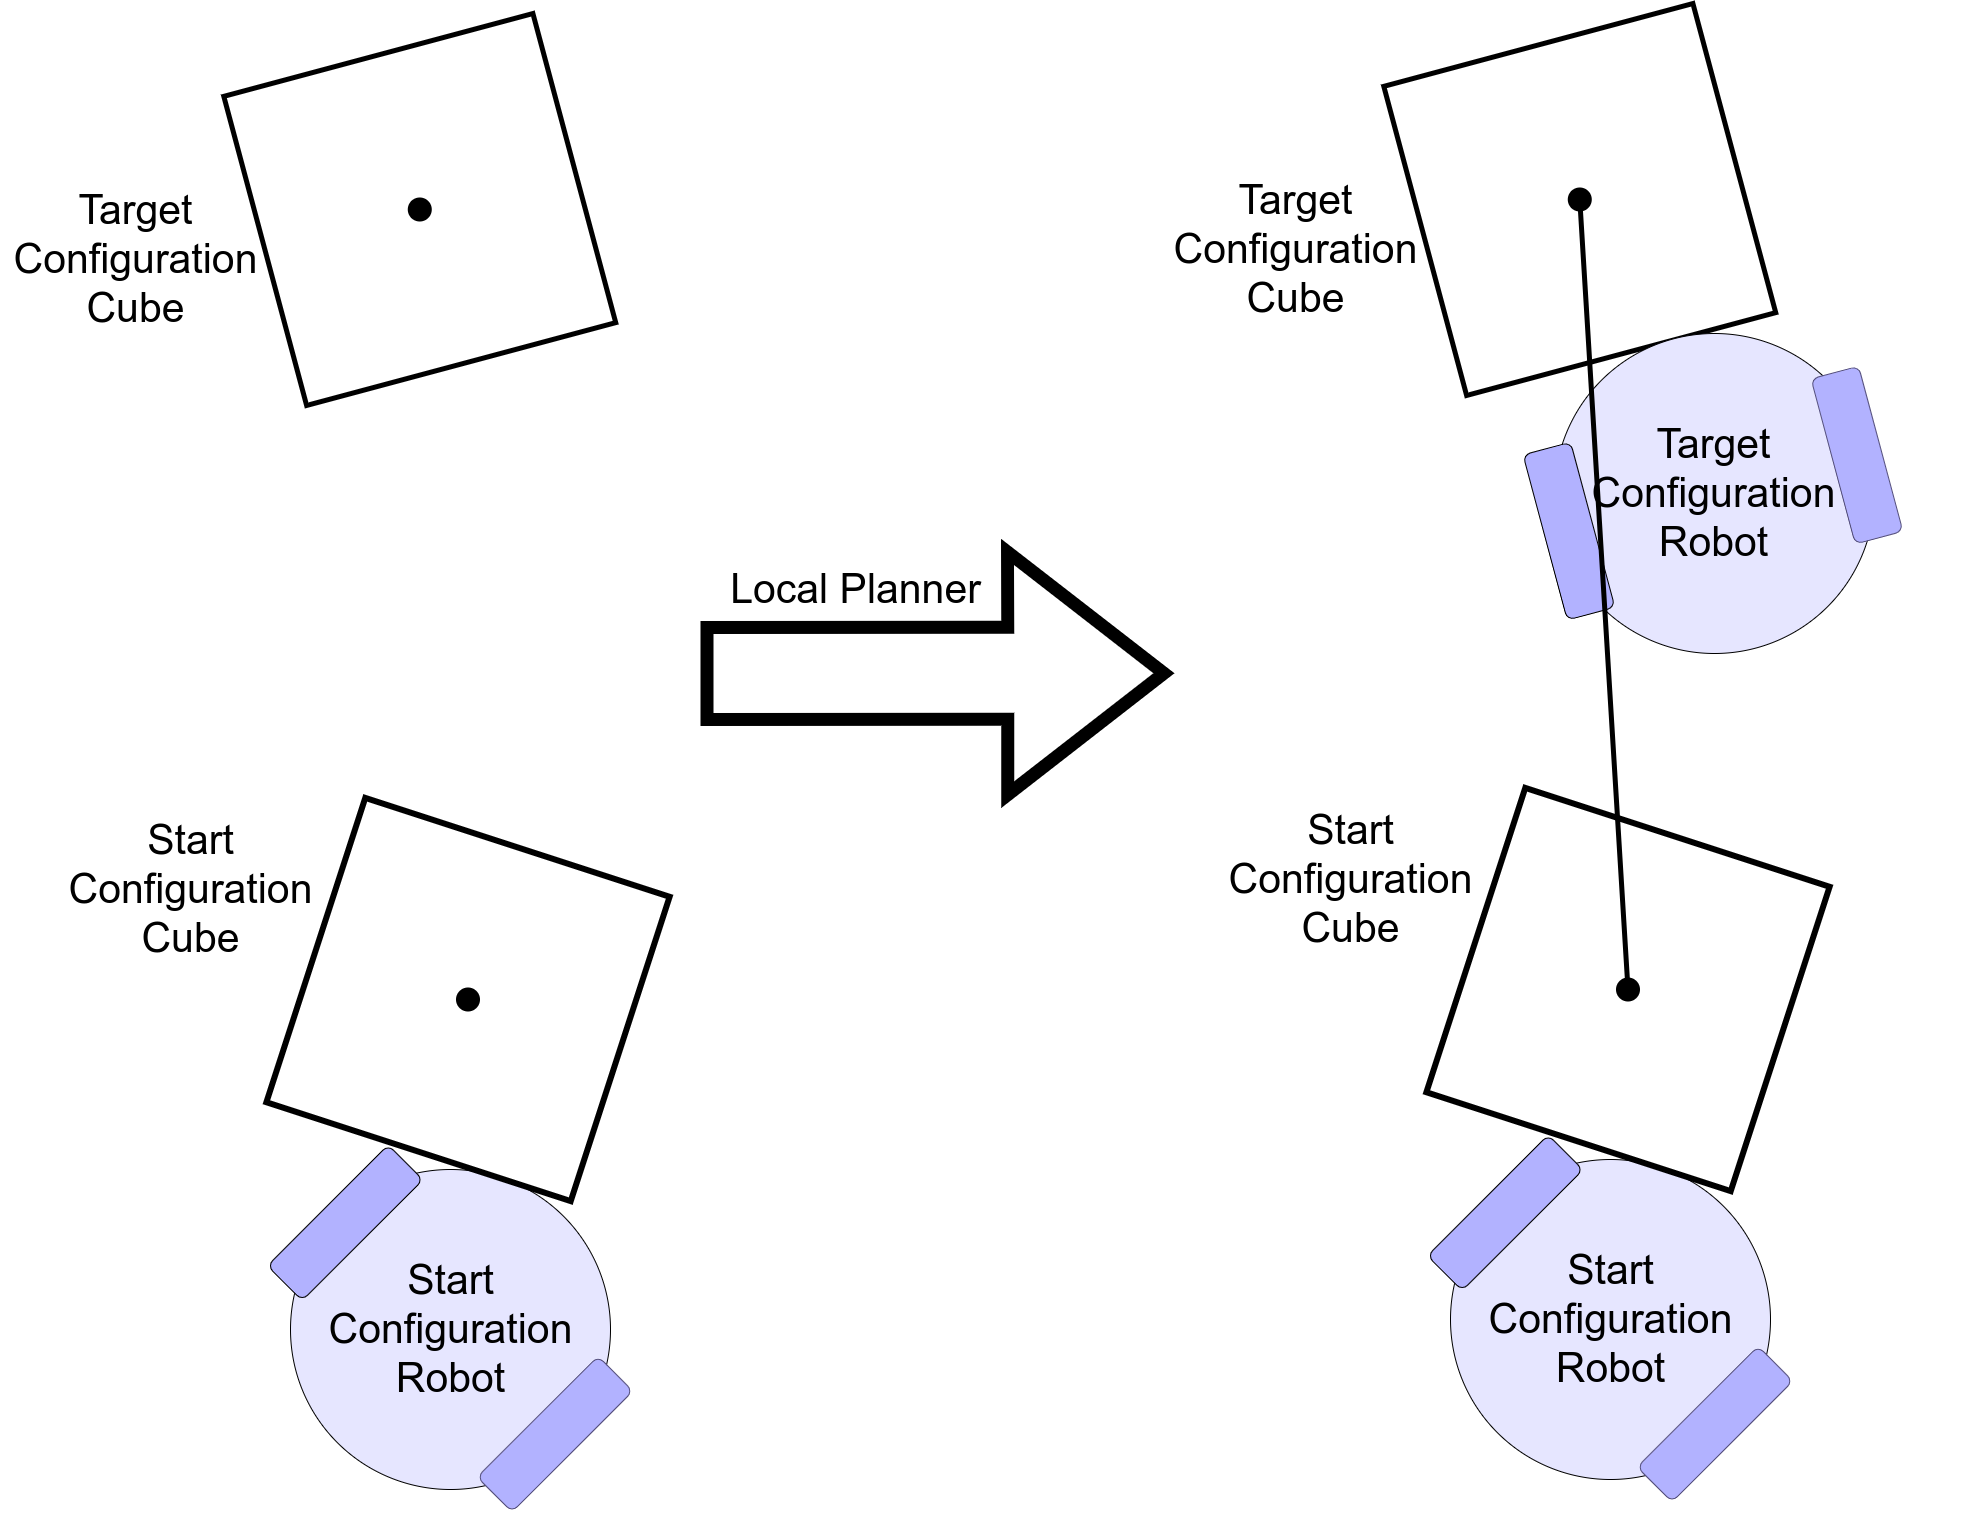
\includegraphics[width=0.6\textwidth]{figures/required_background/manipulation_local_planner}
%     \caption{Generating a new robot configuration whilst adding a sample to the connectivity tree during manipulation planning.}%
%     \label{fig:manipulation_plannig_local_planner}
% \end{figure}
